\documentclass[tikz,border=4pt]{standalone}
\usepackage{xcolor}
\definecolor{journalink}{HTML}{1F1C18}
\begin{document}
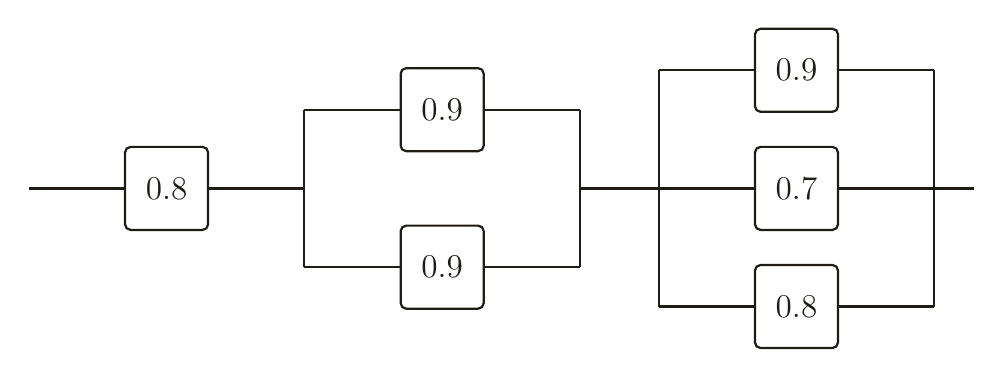
\begin{tikzpicture}[-,auto,node distance=1cm,
  point/.style={coordinate},
  block/.style={draw=journalink, line width=0.8pt, rounded corners=2pt, rectangle, minimum height=3em, minimum width=3em, text=journalink, font=\large},
  every path/.style={draw=journalink, line width=0.8pt}]
\node[point] (0) at (-3,0)  {};
\node[block] (20) at (-1.25,0)  {0.8};
\node[point] (1) at (0.5,0)  {};
\node[point] (2) at (0.5,1)  {};
\node[block] (3) at (2.25,1)  {0.9};
\node[point] (4) at (4,1)  {};
\node[point] (5) at (0.5,-1)  {};
\node[block] (6) at (2.25,-1)  {0.9};
\node[point] (7) at (4,-1)  {};
\node[point] (8) at (4,0)  {};
\node[point] (9) at (5,0)  {};
\node[point] (10) at (5,1.5)  {};
\node[block] (11) at (6.75,1.5)  {0.9};
\node[point] (12) at (8.5,1.5)  {};
\node[point] (13) at (5,-1.5)  {};
\node[block] (14) at (6.75,-1.5)  {0.8};
\node[point] (15) at (8.5,-1.5)  {};
\node[block] (16) at (6.75,0)  {0.7};
\node[point] (17) at (8.5,0)  {};
\node[point] (18) at (9,0)  {};
\draw   (0) -- (20);
\draw   (20) -- (1);
\draw   (1) -- (2);
\draw   (1) -- (5);
\draw   (2) -- (3);
\draw   (3) -- (4);
\draw   (5) -- (6);
\draw   (6) -- (7);
\draw   (4) -- (8);
\draw   (7) -- (8);
\draw   (8) -- (9);
\draw   (9) -- (10);
\draw   (10) -- (11);
\draw   (11) -- (12);
\draw   (9) -- (13);
\draw   (13) -- (14);
\draw   (14) -- (15);
\draw   (9) -- (16);
\draw   (16) -- (17);
\draw   (12) -- (17);
\draw   (15) -- (17);
\draw   (17) -- (18);
\end{tikzpicture}
\end{document}
